\section{Einführung}\label{sec:einfuhrung}
\subsection{Motivation}\label{sec:motivation}
Bildung ist ein wichtiges Element der Persönlichkeitsentwicklung und unter Artikel~26 der allgemeinen Erklärung der Menschenrechte als solches definiert.  Ohne Bildung ist das Ausüben eines gewählten Berufes und das Entwickeln einer Meinung zu komplexen Sachverhalten unmöglich \cite{weitblicker.org2019:online}. Heute sieht sich Bildung durch den digitalen Wandel der letzten Jahre sich noch nie vorher dagewesenen Problemen gegenübergestellt. Wie können Lehrende an Schulen digitale Technik effizient und preiswert im Unterricht einsetzen und so neue Bildungskonzepte erfolgreich in den Lehrplan integrieren? \\ 

Ursprünglich bezeichnet der Begriff Digitalisierung das Umwandeln von Analog nach Digital. Wurde früher Musik auf Schallplatten vertrieben, so wurde diese von der Compact Disc vom Markt verdrängt, welche die Musik auf kleinerem Raum digital abspeichert. Auch wenn der Begriff im Zusammenhang mit Schule längst nicht mehr das Ursprüngliche meint, halte Ich es für sehr wichtig, früher dagewesene Unterrichtskonzepte nicht einfach zu digitalisieren, sondern es erfordert ein Neudenken. Bewährte pädagogische Methoden sollten durch Digitalisierung profitieren sowie neue Konzepte müssen erforscht und entwickelt werden. 

\newpage
\subsection{Ist-Zustand}\label{sec:problemstellung}
%Kurze Zusammenfassung des Forschungsstandes genügend?
Am 04.04.2019 trat die Änderung des Artikel~104c des Grundgesetz für die Bundesrepublik Deutschland in Kraft
und ebnete so den Weg für den von Bund und Ländern beschlossenen Digitalpakt Schule \cite{Art104cG55:online}. 
Dieser Beschluss macht deutlich, dass digitale Kompetenz im Bildungssektor von hoher Bedeutung ist, was von einer Förderungssumme von mindestens 5,5 Milliarden Euro unterstrichen wird. 
Legt man diese Summe auf die ca 40.000 Schulen um, erhält jede Schule einen Durchschnittsbeitrag von 137.000 Euro. Bei ca. 11 Millionen Schülerinnen und Schülern ergibt dies eine Förderungssumme von ca. 500 Euro pro Schülerin bzw. Schüler. 
Einer der Hauptförderungspunkte des Digitalpakt Schule sieht den Ausbau der technischen Infrastruktur
an deutschen Schulen vor, z.B. Bereitstellung von drahtlosen Netzwerken, schnellen Internetzugangspunkten und digitalen Unterrichtsmedien wie interaktiven Whiteboards.
\\ \\
Nach dem Bundesministerium für Bildung und Forschung (BMBF) fördert kein digitales Medium alleine gute Bildung, sondern  immer dahinterstehende pädagogische Konzepte aus einer Vielfalt von Angeboten sind entscheiden \cite{dpakt2019:online}. Ergänzend dazu kritisiert Dennis Horn (Experte für digitale Themen der ARD) den zu starken Fokus auf Hardware und mahnt an, dass zu wenig darüber gesprochen wurde, wie diese denn auch sinnvoll genutzt werden kann \cite{Horn2018:online}. \\ \\
Diese Kritikpunkte wurden auch auf der Podiumsdiskussion der \emph{re:publica 2018} - "`Was kommt in den digitalen Schulranzen?"' angeschnitten. Tobias Hübner, Lehrer und Autor im Bereich Medienistik, zeigt dort ebenfalls auf, dass der Wille Geld auszugeben zu begrüßen sei, es aber an Konzepten und Materialien mangele. Als Lehrer würde er den Investitionsfokus auf Lehrerfortbildung setzen.
\\ \\
Besonders beliebte Hardware an Schulen ist der populäre Tablet Computer \textit{iPad} der Firma Apple inc.  Er wird u.A. an der Oberschule Gehrden bei Hannover von Schülerinnen und Schülern genutzt, wird hier aber von Eltern finanziert \cite{Hett2019}. In der günstigsten Variante liegen die Kosten bereits bei mindestens 449€ \cite{iPadmini65:online} (Stand April 2019), was schon knapp 90\% des Förderungsvolumens pro Schülerin und Schüler ausmachen würde. Als günstigere Alternative ist der Einplatinencomputer \emph{Raspberry Pi} zu nennen (siehe Abbildung \ref{fig:raspberrypi}), welcher bereits für 33~Euro erwerblich ist (Stand April 2019) und genug Rechenkapazitäten bereitstellt um zahlreiche Projekte im Bildungsbereich durchzuführen.

\begin{figure}[H]
	\centering
	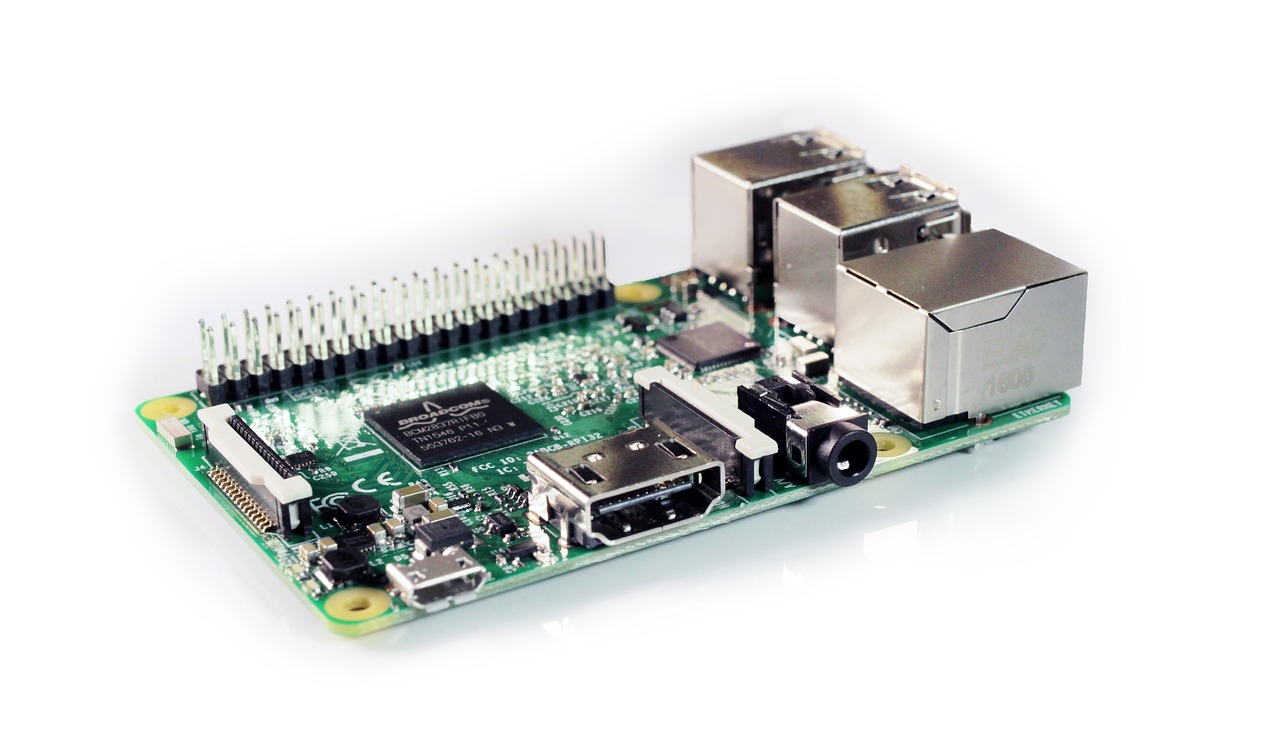
\includegraphics[width=0.9\linewidth]{bilder/raspberry-pi}
	\caption[Raspberry Pi 3 - Einplantinencomputer]{Der Raspberry Pi 3 - Einplantinencomputer \cite{PixaPi2016}}
	\label{fig:raspberrypi}
\end{figure}

Mit Touchscreenmodul und Schutzhülle liegt der Preis insgesamt bei ca. 150~Euro, was immer noch weniger als die Hälfte des Fördervolumens beträgt.



\paragraph{Besuch der Grundschule am Rüdesheimer Platz Berlin}\label{sec:grundschulebesuch}
Im Rahmen der Vorrecherche zu dieser Arbeit wurde einem Unterrichtstag in 
einer Jahrgangsübergreifenden (JüL) Klasse 1 bis 3 an der Grundschule am Rüdesheimer Platz beigewohnt um ein differenzierteres 
Bild der gegenwärtigen Lern- und Digitalisierungssituation an einer Berliner Schule zu bekommen. An dieser Stelle eine große Dankaussagung an Frau Wewer, Grundschullehrerin, welche diese Erfahrung möglich gemacht hat und in einem anschließenden Gespräch das Interesse an einer kostengünstigen und einfach nutzbaren Lösung zur Unterstützung von interaktiven Unterrichtsmethoden unterstrichen hat.
\newpage
\subsection{Aufbau der Arbeit}

Im Anschluss an dieses Kapitel folgt die Formulierung einer \hyperref[sec:zielsetzung]{\textbf{Zielsetzung}}. Darauf folgend werden \hyperref[sec:grundlagen]{\textbf{Grundlagen}} erörtert. Dies umfasst die Themengebiete Digitalisierung an Schulen und einen Überblick über Webtechnologie. Ersteres ist für den späteren potentiellen Einsatz der Software maßgebend, letzteres bildet das technologische Fundament, welches die Implementierung erst möglich macht. Anschließend wird in Kapitel \hyperref[sec:analyse]{\textbf{Analyse}} ein Vergleich zwischen existierenden kommerziellen und nicht-kommerziellen Plattformen gezogen. Darauf aufbauend folgt eine Anforderungs- und Systembeschreibung. Im darauffolgenden Kapitel \hyperref[sec:konzept]{ \textbf{Konzept}} wird ebendieses erörtert und darauffolgend der Prozess der \hyperref[sec:implementierung]{\textbf{Implementierung}} beschrieben. In einer folgenden \hyperref[sec:auswertung]{\textbf{Auswertung}} werden die Ergebnisse mit den geplanten Zielen verglichen und ein Fazit gezogen. Schlussendlich wird im letzten Abschnitt ein \hyperref[sec:ausblick]{\textbf{Ausblick}} formuliert, welcher die Zukunft des Projekts betrifft. 
\\ \\
{\underline{Genderhinweis:} Aus Gründen der Lesbarkeit wurde in dieser Arbeit die männliche Form gewählt, nichtsdestoweniger beziehen sich die Angaben auf Angehörige beider Geschlechter.  



\newpage


   
